\section{Evaluating the performance of the proposed method}
\label{sec:rul_eval}

In this section we evaluate the performance of the proposed method. The architecture of the \gls{mlp} to be used here is described in Table \ref{table:proposed_nn} and will be used throughout this section.  The \gls{mlp} was trained $10$ times for $200$ epochs each and tested in each subset of the \gls{cmaps} dataset.

For the first experiment, the combinations of window size $n_w$, window stride $n_s$ and early \gls{rul} $R_e$ are presented in Table \ref{table:data_params_de}.

\begin{table}[!htb]
\centering
\begin{tabular}{l r r r l}
	\hline
	 Dataset & $n_w$ &  $n_s$ & $R_e$\\
  	\hline
  	FD001 & 30 & 1 & 128\\
  	FD002 & 20 & 2 & 134\\
  	FD003 & 30 & 1 & 128\\
  	FD004 & 18 & 2 & 134\\
  	\hline
\end{tabular}
\caption{Data-related parameters for each subset as obtained by \gls{de}.}
\label{table:data_params_de}
\end{table}  

The obtained results for $f(v)$ using the above setting are depicted in Table \ref{table:results_ann_de}. Notice that the performances obtained for datasets FD001 and FD002 improved, this is due to the fact that this time the \gls{mlp} was trained for more epochs, thus obtaining better results.

\begin{table}[!htb]
\centering
\begin{tabular}{l | r r r r | r r r r}
	\hline	
	& \multicolumn{4}{| c}{RMSE} & \multicolumn{4}{| c}{RHS} \\
	Data Subset & min & max & avg & STD & min & max & avg & STD\\
  	\hline
  	FD001 & 14.87 & 15.08 & 14.94 & 0.06 &3.65 & 3.99 & 3.86 & 0.10\\
  	FD002 & 28.67 & 31.60 & 29.54 & 0.91 & 49.15 & 92.52 & 61 & 13.52\\
  	FD003 & 14.55 & 16.21 & 15.05 & 0.52 & 3.88 & 4.54 & 4.17 & 0.22\\
  	FD004 & 32.54 & 37.703 & 34.08 & 1.43 & 48.35 & 79.33 & 59.60 & 10.26\\
  	\hline
\end{tabular}

\caption{Scores for each dataset using the data-related parameters obtained by \gls{de}.}
\label{table:results_ann_de}
\end{table}

Next, the possibility of using a single set of data-related parameters for all the subsets is explored. For this experiment the $n_w$ is fixed for all of the four datasets, given that the maximum allowable window size for all datasets is $18$. Hence, the data-related chosen parameters are $v=(18, 2, 18)$, the results obtained are shown in Table \ref{table:results_ann_1}. 

\begin{table}[!htb]
\centering
\begin{tabular}{l | r r r r | r r r r}
	\hline	
	& \multicolumn{4}{| c}{RMSE} & \multicolumn{4}{| c}{RHS} \\
	Data Subset & min & max & avg & STD & min & max & avg & STD\\
  	\hline
  	FD001 & 17.58 & 18.56 & 17.82 & 0.29 & 8.26 & 9.18 & 8.59 & 0.28\\
  	FD002 & 29.48 & 31.92 & 30.15 & 0.75 & 65.83 & 104.37 & 75.73 & 11.54\\
  	FD003 & 17.35 & 19.99 & 18.20 & 0.72 & 6.25 & 16.09 & 8.27 & 2.86\\
  	FD004 & 32.91 & 37.28 & 34.45 & 1.41 & 48.90 & 77.93 & 59.60 & 9.65\\
  	\hline
\end{tabular}
\caption{Scores for each dataset using the single set of data-related parameters.}
\label{table:results_ann_1}
\end{table}

As can be observed, performance is decreased for subsets FD001/FD003, this indicates that larger window sizes are beneficial for this regression problem. Figures \ref{fig:scores_rmse} and \ref{fig:scores_rhs} show a comparison of how the scores are affected for each dataset by changing the data-related parameters to make use of 2 and 1 sets of them.

\begin{figure}[!htb]
\centering
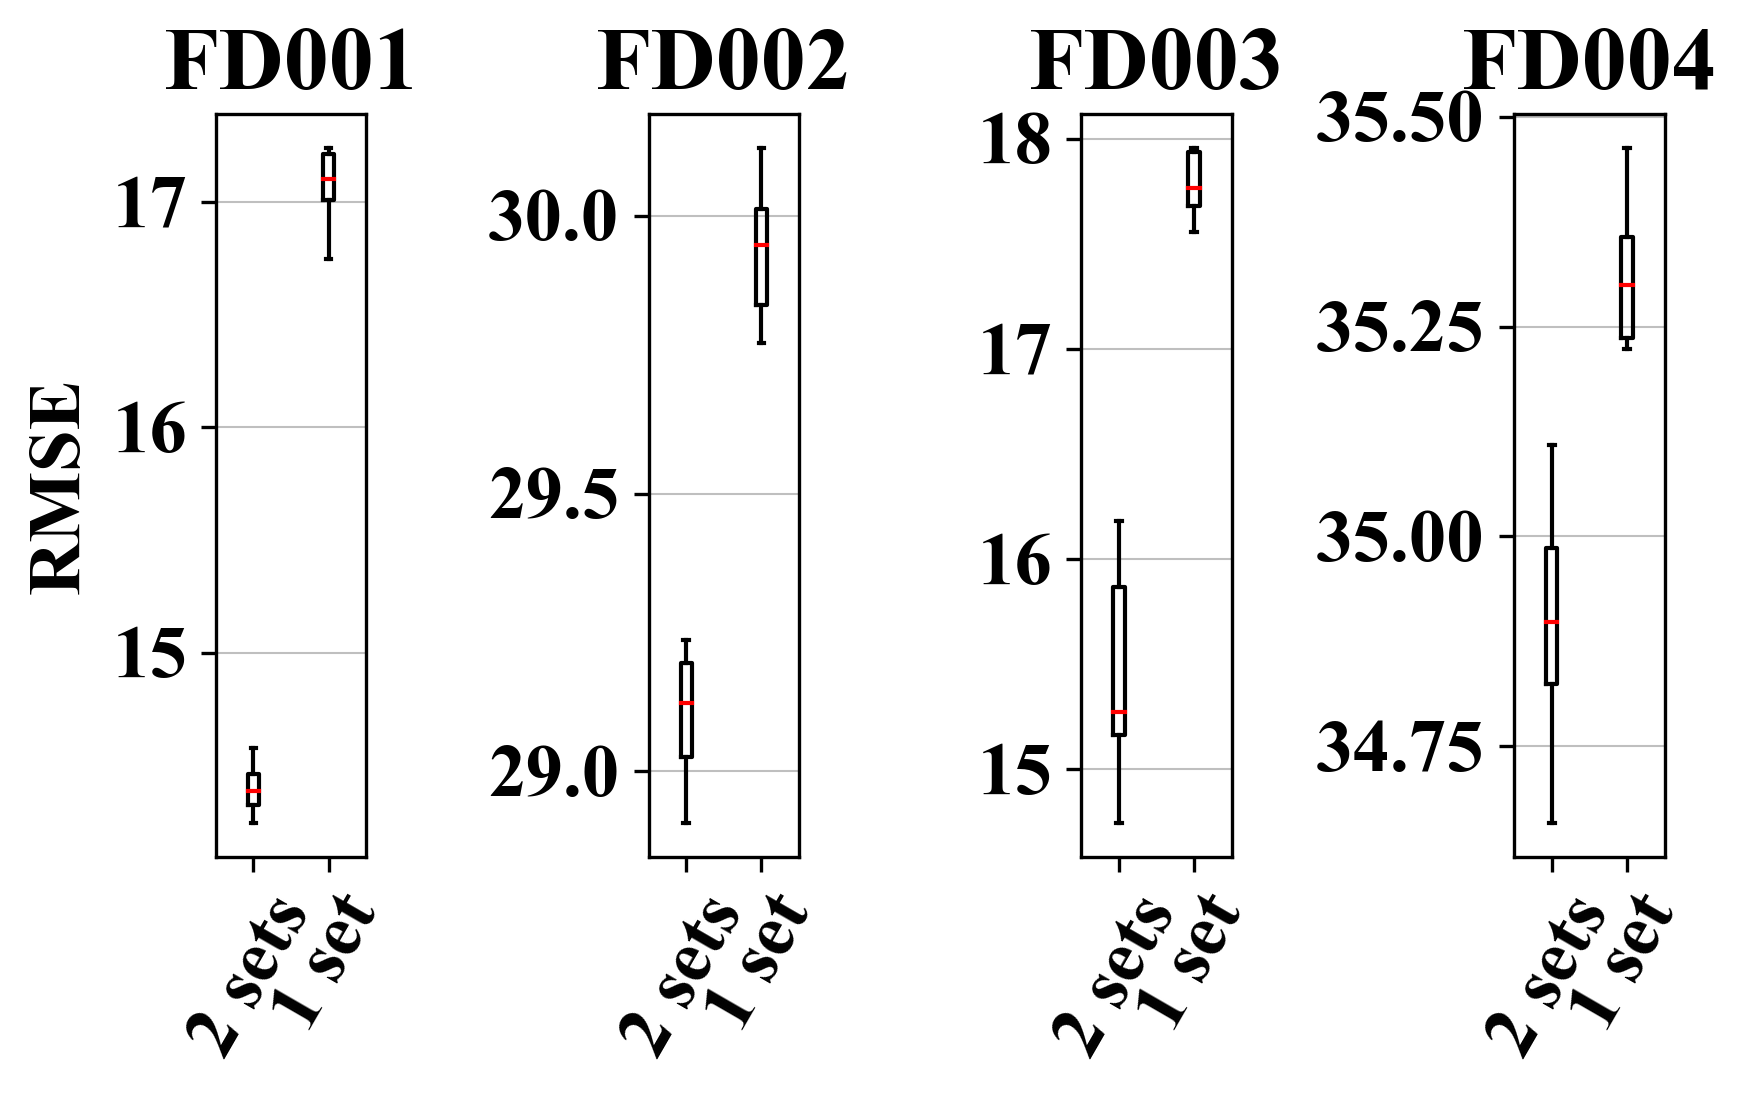
\includegraphics[width=0.7\textwidth]{../img/rmse_comparisson.png}
\caption{Comparison of \gls{rmse} results for different sets of data-related parameters.}
\label{fig:scores_rmse}
\end{figure}

\begin{figure}[!htb]
\centering
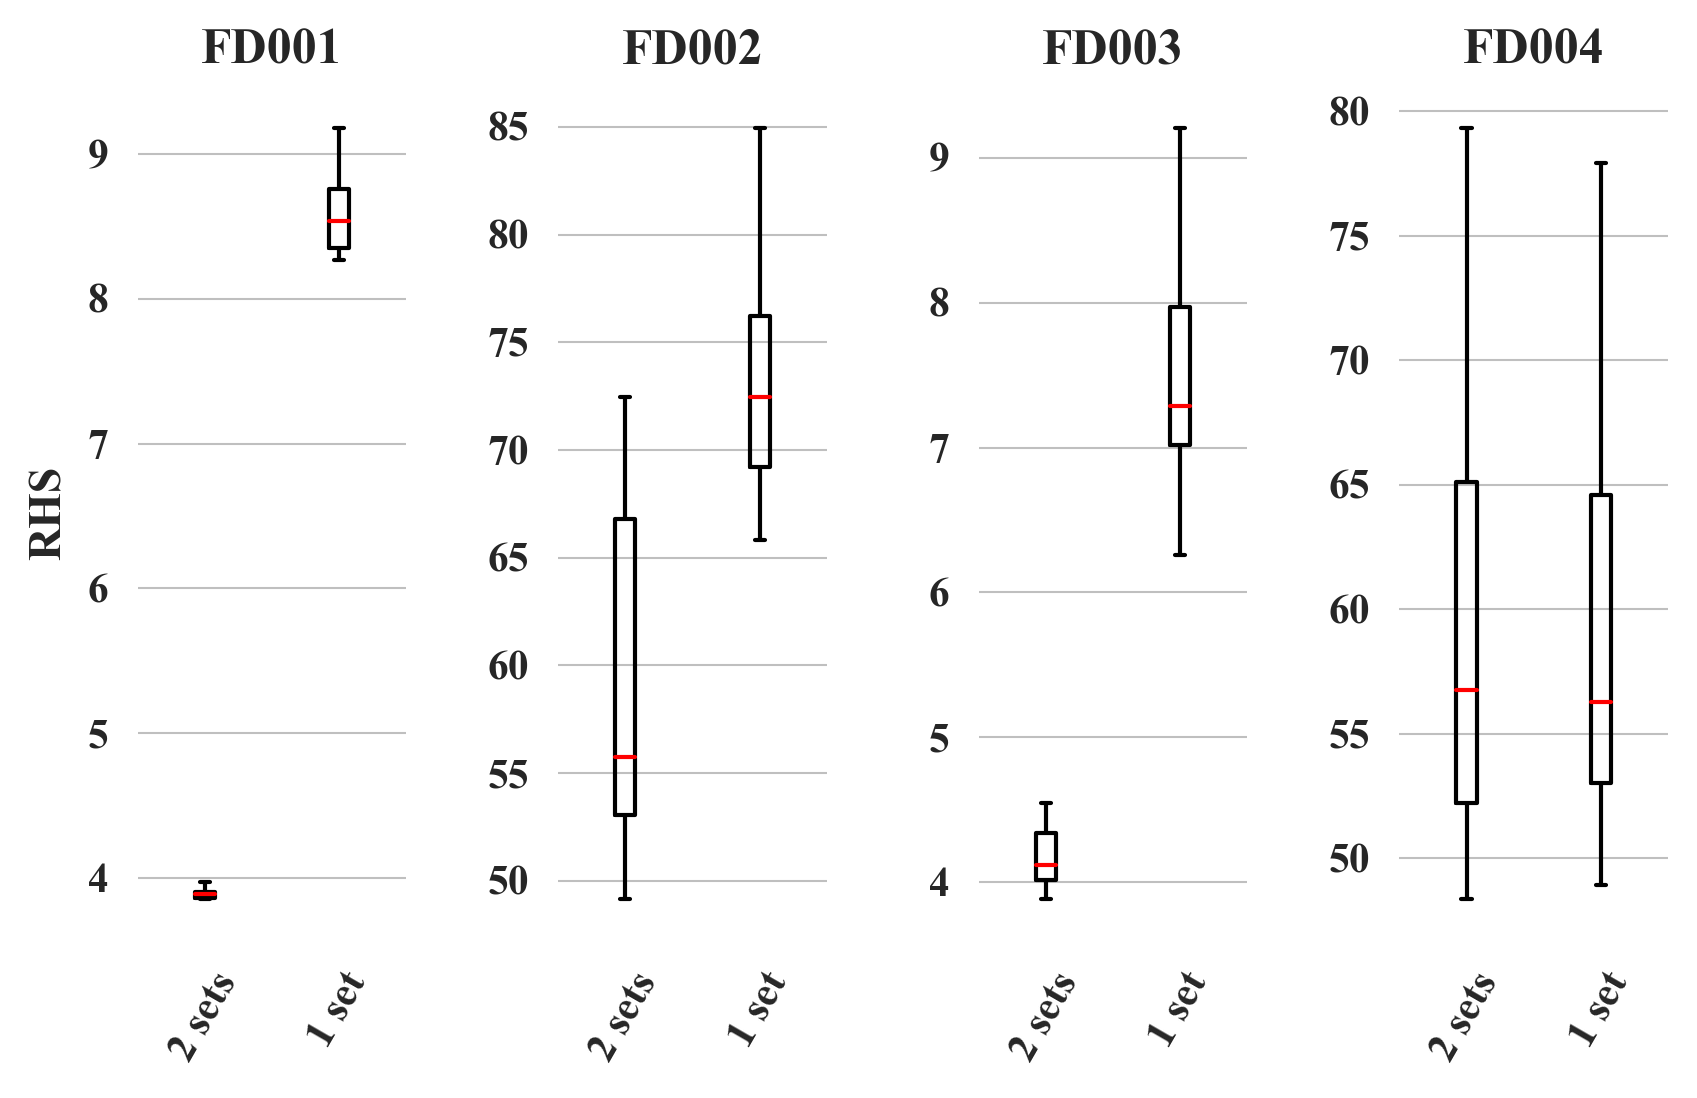
\includegraphics[width=0.7\textwidth]{../img/rhs_comparisson.png}
\caption{Comparison of \gls{rhs} results for different sets of data-related parameters.}
\label{fig:scores_rhs}
\end{figure}

\subsection{Comparison with other approaches}

In this section the performance of the proposed method is compared against other state-of-the-art methods. Most of the presented methods in this section have only reported results on the test set FD001 in terms of $e_{rms}$, the results are displayed in Table \ref{table:results_comparison}. The $e_{rms}$ value of the proposed method in Table \ref{table:results_comparison} is the mean value of 10 independent runs. The remainder of the values are identical to those reported in their respective original papers.

\begin{table}[!htb]
\centering
\begin{tabular}{l | r r r r | r r r r}
	\hline	
	Method & $e_{rms}$ \\
  	\hline
  	ESN trained by Kalman Filter \citep{Peng2012} & 63.45\\
  	Support Vector Machine Classifier \citep{Louen2013} & 29.82\\
  	Time Window Neural Network \citep{Lim2016} & 15.16\\
  	Multi-objective deep belief networks ensemble \citep{Zhang2016} & 15.04\\
  	Deep Convolutional Neural Network \citep{Babu2016} & 18.45\\
  	\textbf{Proposed method with $n_w = 30$, $n_s=1$ and $R_e = 128$} & 14.87\\
  	\hline
\end{tabular}
\caption{Performance comparisons of the proposed method and the latest related papers on the \gls{cmaps} dataset.}
\label{table:results_comparison}
\end{table}

Based on the results, the proposed method performs better than the majority of the compared methods when taking into consideration the whole dataset FD001. Two methods come close to the performance of the presented approach in this paper, namely the time window \gls{ann} \citep{Lim2016} and the Networks Ensemble \citep{Zhang2016}. While the performance of both methods comes close to the results presented in this paper, the presented approach is computationally more efficient. Furthermore, the framework proposed in here is simple to understand and implement, robust, generic and light-weight, features we believe are important to highlight when comparing the proposed method against other state-of-the-art approaches.

